\documentclass[oneside, draft]{epstfg}

\usepackage{lipsum}
\usepackage[numbers]{natbib}
\usepackage{fancysprefs}
\usepackage{booktabs}
\usepackage{wrapfig}
\usepackage{enumitem}


\usepackage{tikz}

\usetikzlibrary{arrows}
\usetikzlibrary{patterns}
\usetikzlibrary{intersections}
\usetikzlibrary{calc}
\usetikzlibrary{fadings}

\definecolor{palette1}{HTML}{1B9E77}
\definecolor{palette2}{HTML}{D95F02}
\definecolor{palette3}{HTML}{7570B3}
\definecolor{palette4}{HTML}{E7298A}
\definecolor{palette5}{HTML}{66A61E}
\definecolor{palette6}{HTML}{E6AB02}
\definecolor{palette7}{HTML}{A6761D}
\definecolor{palette8}{HTML}{666666}

\tikzstyle{vnlin}=[rectangle, inner sep=0pt, minimum height=6pt, minimum width=0pt, draw, fill=black]
\tikzstyle{hnlin}=[rectangle, inner sep=0pt, minimum height=0pt, minimum width=6pt, draw, fill=black]
\tikzset{>=latex}

\bibliographystyle{abbrv}

\title[spa]{Monitorización, captura y almacenamiento inteligente de tráfico de red a 40Gbps}
\title[eng]{Monitoring, capture and smart storage of network traffic at 40 Gbps}
\author{Guillermo Julián Moreno}
\tutor{Francisco Gómez Arribas}
\date[spa]{Mayo 2016}
\date[eng]{May 2016}
\group[spa]{HPCN}
\group[eng]{HPCN}
\department[spa]{Departamento}
\department[eng]{Department}

\setdegreeDouble

\begin{abstract}[spa]
\lipsum[1]
\end{abstract}

\begin{abstract}[eng]
\lipsum[2]
\end{abstract}

\keywords[spa]{keyword, comma, separated, list}
\keywords[eng]{keyword, comma, separated, engl}

\newacronym[longplural = {Centros de Proceso de Datos}]{cpd}{CPD}{Centro de Proceso de Datos}
\newacronym{gbps}{Gbps}{Gigabits por segundo}
\newacronym{nic}{NIC}{Tarjeta de Interfaz de Red}
\newacronym{irq}{IRQ}{petición de interrupción}

\newglossaryentry{10gbe}{name = {10 GbE}, description = {Estándares de transmisión de datos sobre Ethernet a 10 gigabits por segundo}}
\newglossaryentry{NAPI}{name = {NAPI}, description = {``New API'', una API de Linux desarrollada para mitigar interrupciones en \textit{drivers} de red y mejorar el rendimiento bajo condiciones de alta carga}}

\newglossaryentry{driver}{
	name = {Driver},
	text ={\textit{driver}},
	description = {También llamado controlador de dispositivo, es un programa que permite al sistema operativo interactuar con un periférico \textit{hardware}}}

\newglossaryentry{jumbo}{
	name = {Paquete jumbo},
	text={paquete jumbo},
	description = {Paquetes Ethernet de tamaño superior a 1500 bytes}}

\newglossaryentry{DMA}{
	name = {DMA},
	description = {Direct Memory Access, un sistema que permite a los periféricos acceder directamente a la memoria del sistema}
}

\begin{document}

\selectlanguage{spanish}

\frontmatter

\maketitle[spa]
\maketitle[eng]

\makeinnertitle[spa]
\makeinnertitle[eng]

\makeabstract[spa]
\makeabstract[eng]

\tableofcontents
\clearsidepage
\listoftables
\clearsidepage
\listoffigures
\clearsidepage

\mainmatter

\chapter{Introducción y motivación}

Durante los últimos años, las necesidades de ancho de banda de Internet se han ido multiplicando a una velocidad difícil de imaginar en su momento. Muchos \glspl{cpd} ya han desplegado redes \gls{10gbe}, y los dispositivos capaces de funcionar a 40 \gls{gbps} o incluso a 100 \gls{gbps} ya están disponibles comercialmente.

Por supuesto, junto con las nuevas redes de alta velocidad llega la necesidad de monitorizarlas, ya sea para diagnosticar problemas, detectar intrusiones o asegurar un nivel de calidad de servicio. Sin embargo, los sistemas operativos modernos no están totalmente preparados para el manejo de estas velocidades. Incluso para \gls{10gbe} se hacen necesarias configuraciones específicas \cite{leitao2009tuning} que permitan al sistema alcanzar las tasas que ofrece el \textit{hardware}.

Para sortear las limitaciones de los sistemas operativos en este sentido son necesarias soluciones específicas y dedicadas.

\todo{Pequeño overview del estado del arte.}

Dos aspectos que muchas soluciones de monitorización no contemplan es el de marcado de paquetes o \textit{timestamping} y el del orden de captura. A 40 Gbps, el tiempo entre paquetes puede llegar a ser de 13 nanosegundos\footnote{Tomando paquetes de tamaño mínimo, 64 bytes, y añadiendo el \textit{interframe gap} de 8 bits.}. Una recepción desordenada o imprecisiones mínimas en las marcas de tiempo pueden ser decisivas para que una herramienta de análisis detecte o ignore anomalías en el tráfico; o para que dé falsos positivos a raíz de fallos en la captura. Teniendo en cuenta que estos problemas ya los introducen las propias redes y sistemas a monitorizar, es necesario reducirlos todo lo posible en el lado de la captura.

\section{Objetivos}

Este trabajo se plantea resolver el problema de la monitorización de tráfico en redes 40 GbE, ampliando el sistema de captura HPCAP \cite{MorenoTFM2012}, de Víctor Moreno. Para ello, los \todo{focos?} serán los siguientes:

\begin{itemize}
\item Estudiar los límites de la arquitectura ya existente de HPCAP e identificar los puntos de mejora.
\item Plantear una solución que permita la captura de tráfico a tasa de línea junto con marcas de tiempo precisas.
\item Desarrollar métodos que hagan posible el almacenamiento de información sobre el tráfico que pueda ser analizada posteriormente.
\end{itemize}

\chapter{Estado del arte}

HPCAP, artículo de Javier de 40Gbps. DPDK, sockets de acceso directo (PF\_LINUX?).

\section{Funcionamiento de un \textit{driver} de red: ¿Qué hay que cambiar para alto rendimiento?}
\label{sec:EstadoArte:Funcionamiento}

\begin{figure}[hbtp]
\centering
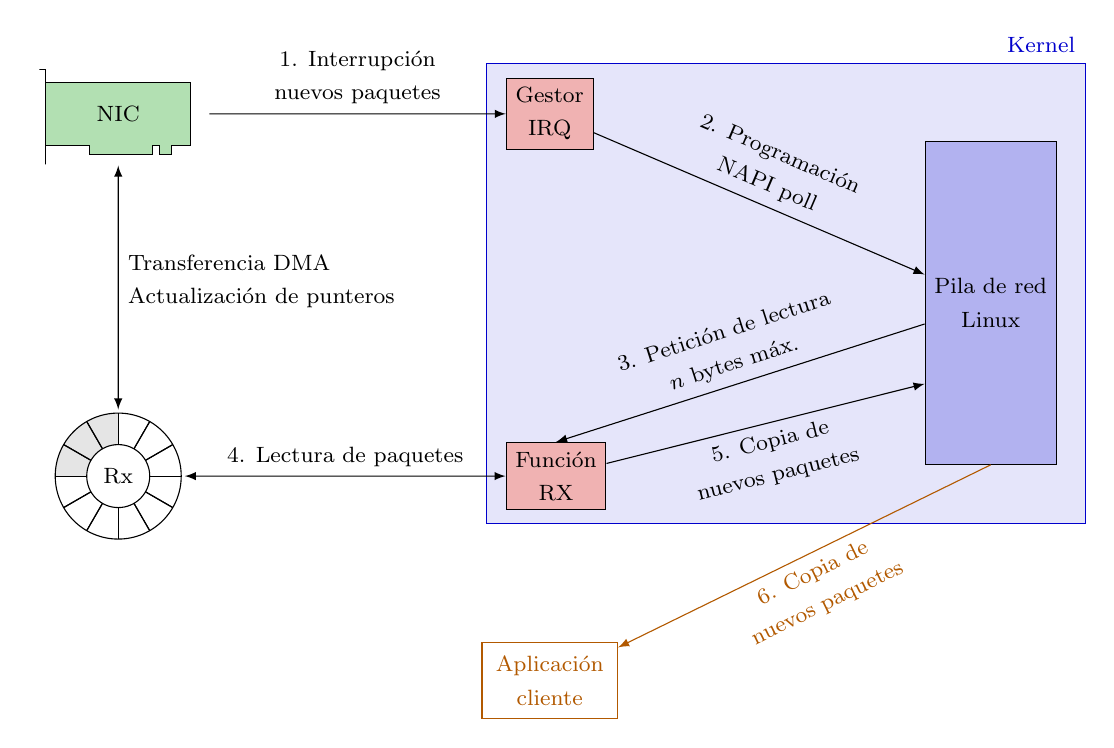
\begin{tikzpicture}[font = {\fontsize{8pt}{12}\selectfont}, scale = 0.8]
\begin{scope}[yshift = 4cm]
\draw[fill = green!60!black, fill opacity = 0.3] (-0.1, 1.2) -- (0, 1.2) -- (0,-0.3) -- (0,0) -- (0.7,0) -- (0.7,-0.15) -- (1.7, -0.15) -- (1.7, 0) -- (1.8, 0) -- (1.8, -0.15) -- (2, -0.15) -- (2,0) -- (2.3, 0) -- (2.3, 1) -- (0,1) -- (0, 1.2) -- cycle ;

\node[rectangle, minimum width = 2.3cm, minimum height = 1cm] (NIC) at (1.15, 0.5) {NIC};
\end{scope}

\draw[blue!80!black, fill = blue!80!black, fill opacity = 0.1] (7, 5.3) rectangle (16.5, -2);
\node[blue!80!black] at (15.8, 5.6) {Kernel};


\node[draw, fill = red!80!black!30!white, align = center] (IRQ) at (8, 4.5) {Gestor \\ IRQ};
\node[draw, fill = blue!80!black!30!white, minimum height = 4.1cm, minimum width = 1.5cm, align = center] (KRN) at (15, 1.5) {Pila de red \\ Linux};
\node[draw, align = center, fill = red!80!black!30!white] (POLL) at (8.1, -1.25) {Funci\'on \\ RX};

\node[draw, orange!70!black, align = center, inner sep = 5pt] (APP) at (8, -4.5) {Aplicaci\'on \\ cliente};

\coordinate (KRN-Mid) at ($(KRN.west)!0.5!(KRN.south west)$);

\begin{scope}[xshift = 1.15cm, yshift = -1.25cm, rotate = 90]
\fill[gray!20!white] (0,0) -- (0,1) arc (90:0:1cm) -- cycle;
\foreach \x in {0, 30, ..., 360}
	\draw ({cos(\x)}, {sin(\x)}) -- ({-cos(\x)}, {-sin(\x)});
\draw (0,0) circle [radius = 1cm];
\draw[black, fill = white] (0,0) circle [radius = 0.5cm]; % Poor man's \clip for intersecting regions
\node[circle, inner sep = 0.45cm] (RNG) at (0,0) {Rx};
\end{scope}

\draw[->] (NIC) --
	node[midway, above, align = center, sloped] {1. Interrupci\'on \\ nuevos paquetes}
	(IRQ);

\draw[->] (IRQ) --
	node[midway, above, sloped, align = center] {2. Programaci\'on \\ NAPI poll}
	(KRN);

\draw[->] (KRN) --
	node[midway, above, sloped, align = center] {3. Petici\'on de lectura \\ $n$ bytes m\'ax.}
	(POLL.north);

\draw[<->, shorten <= 0.15cm] (NIC) --
	node[midway, right, align = left] {Transferencia DMA \\ Actualizaci\'on de punteros}
	(RNG);

\draw[<->] (POLL) -- node[midway, above, align = center, sloped] {4. Lectura de paquetes}
	(RNG);

\draw[->] (POLL) --
	node[midway, below, align = center, sloped] {5. Copia de \\ nuevos paquetes}
	(KRN-Mid);

\draw[<-, orange!70!black] (APP) --
	node[midway, below, sloped, align = center] {6. Copia de  \\ nuevos paquetes}
	(KRN.south);
\end{tikzpicture}

\caption[Funcionamiento de un \textit{driver} de red en Linux]{Esquema del funcionamiento de un \gls{driver} de red en Linux. En rojo, las funciones pertenecientes al \gls{driver}.}
\label{fig:LinuxNetworkStack}
\end{figure}

A grandes rasgos, el funcionamiento de un \textit{\gls{driver}} de red en Linux es el que aparece en la \fref{fig:LinuxNetworkStack}. Cuando la \gls{nic} recibe nuevos paquetes, emite una \gls{irq} que es recibida por la función correspondiente configurada por el \gls{driver}. Éste se comunica con la pila de red del \textit{kernel} de Linux, más concretamente con el subsistema \gls{NAPI} \cite{NAPI}, avisando de la disponibilidad de nuevos paquetes. Además, desactivará las interrupciones de la tarjeta hasta que no se hayan leído todos los paquetes pendientes, para mejorar así el rendimiento.

El subsistema \gls{NAPI} programará una llamada a la función de recepción del \gls{driver} en función de la carga del sistema, pidiendo la lectura de hasta un cierto máximo de bytes. Cuando esa llamada se realice, el \gls{driver} leerá de una región de memoria los paquetes que la tarjeta haya copiado a través de transferencias DMA, y los transferirá a la pila de red de Linux, que a su vez los gestionará y distribuirá a las aplicaciones cliente correspondientes.

Si bien esta arquitectura es muy efectiva para un sistema de propósito general, tiene varias desventajas como sistema de captura de alto rendimiento. Por un lado, se introduce una cierta latencia al tener que esperar a la primera interrupción y a la llamada correspondiente del subsistema NAPI para empezar a leer los paquetes del anillo de recepción de la tarjeta. Por otra, se realizan dos copias redundantes: del anillo de recepción a la pila de red de Linux y de ésta a la aplicación cliente.

\subsection{HPCAP}

\chapter{Desarrollo e implementación}

\section{Arquitectura de los \textit{drivers} originales}
\label{sec:ArquitecturaOriginal}

\begin{figure}[btp]
\centering
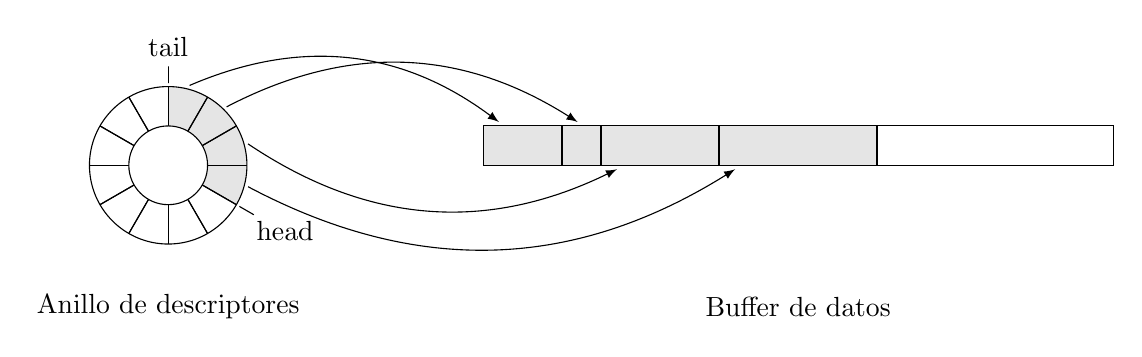
\begin{tikzpicture}
\fill[gray!20!white] (0,0) -- (0,1) arc (90:-30:1cm) -- cycle;
\foreach \x in {0, 30, ..., 360}
	\draw ({cos(\x)}, {sin(\x)}) -- ({-cos(\x)}, {-sin(\x)});
\draw (0,0) circle [radius = 1cm];
\draw[black, fill = white] (0,0) circle [radius = 0.5cm]; % Poor man's \clip for intersecting regions

\node[vnlin, label = {above:tail}] at (0,1.15) {};

\node[hnlin, label = {below right:head}, rotate = -30] at ({1.15 * cos(-30)}, {1.15 * sin(-30)}) {};

\node at (0, -1.8) {Anillo de descriptores};
\node at (8, -1.8) {Buffer de datos};

\fill[gray!20!white] (4, 0) rectangle (9, 0.5);
\draw (4, 0) rectangle (12,0.5);

\draw[thick] (5, 0) -- (5, 0.5);
\draw[thick] (5.5, 0) -- (5.5, 0.5);
\draw[thick] (7, 0) -- (7, 0.5);
\draw[thick] (9, 0) -- (9, 0.5);

\draw[->] ({1.05 * cos(75)}, {1.05 * sin(75)}) to [bend left] (4.2, 0.55);
\draw[->] ({1.05 * cos(45)}, {1.05 * sin(45)}) to [bend left] (5.2, 0.55);
\draw[->] ({1.05 * cos(15)}, {1.05 * sin(15)}) to [bend right] (5.7, -0.05);
\draw[->] ({1.05 * cos(-15)}, {1.05 * sin(-15)}) to [bend right] (7.2, -0.05);

\end{tikzpicture}

\caption[Esquema del anillo de descriptores para recepción de paquetes]{Esquema del anillo de descriptores para la recepción de paquetes. Cada descriptor tiene un puntero a los datos del paquete recibido y un campo que marca si el descriptor tiene o no datos. En gris, los datos y descriptores listos para ser leídos por el \gls{driver}.}
\label{fig:DriverRings}
\end{figure}

Para poder adaptar HPCAP a las \glspl{nic} de 40 Gbps de Intel y Mellanox es necesario utilizar los \glspl{driver} originales de los fabricantes y modificarlos para que sea el código de HPCAP el encargado de la recepción. Esto implica conocer su funcionamiento no sólo a grandes rasgos (\fref{sec:EstadoArte:Funcionamiento}), sino también las rutinas de comunicación con el \textit{hardware} y de reserva de recursos de esos \glspl{driver} originales.

A pesar de ser de fabricantes distintos, los dos \glspl{driver} siguen el mismo proceso para inicializarse y para la recepción de paquetes. Cuando el \gls{driver} se inserta en el sistema Linux, lee los parámetros de configuración de la línea de comandos y empieza a reservar recursos acorde a esos parámetros. Entre esos recursos están las regiones de memoria de los anillos de recepción, donde la \gls{nic} escribirá los paquetes recibidos; y estructuras en memoria compartida entre \textit{software} y \textit{hardware}, de donde se leerán datos como los descriptores de paquetes y los punteros de cabecera y cola del anillo.

El anillo de descriptores es la estructura de datos que permite la transferencia de paquetes desde la \gls{nic} al \gls{driver}. Cada descriptor de paquete es una estructura de tamaño fijo que contiene una variable con el estado del descriptor, con los marcadores que determinan si tiene datos, si ha tenido algún error o si es parte de un \gls{jumbo}; y un puntero a los datos del paquete de red correspondiente, que han sido copiados a la memoria del sistema por la \gls{nic}.

Este anillo se comporta como una cola, aunque el acceso se realiza de manera distinta. El puntero de cabecera, \textit{head}, que marca hasta dónde hay paquetes pendientes de leer, no se actualiza por la \gls{nic} al enviar nuevos paquetes al sistema. En su lugar, para comprobar si hay o no nuevos paquetes por leer, el \gls{driver} simplemente lee el campo de estado del siguiente descriptor de paquete para saber si tiene datos o no.

La rutina de recepción, llamada por el subsistema \gls{NAPI}, va leyendo ese anillo de descriptores y enviando los nuevos paquetes que encuentra al sistema operativo, que se encargará de repatirlos a su destino correspondiente.

Una vez que los paquetes se han leído, no sólo hay que actualizar el puntero de cola, sino también notificar al sistema \gls{DMA} de que la memoria que usaban queda libre para su uso por la tarjeta. Realizar esta operación paquete por paquete introduce un coste adicional que se puede ahorrar acumulando varias operaciones que se realizan de una vez, aunque no deben acumularse demasiadas para evitar que la \gls{nic} se quede sin descriptores donde copiar nuevos paquetes y los descarte.

Por lo tanto, para que HPCAP funcione con estos \glspl{driver}, la principal modificación a hacer es sustituir la rutina de recepción original. Para ello, se evita el registro de la interfaz en el subsistema \gls{NAPI}, se desactivan las interrupciones de la \gls{nic}, y se lanzan los hilos de recepción de HPCAP cuando el resto del \gls{driver} se haya inicializado correctamente.

\section{Recepción a 40 Gbps}

Tal y como se comentaba en la introducción, la recepción a 40 Gbps es un desafío importante por las restricciones de tiempo. A esta tasa, los paquetes pueden llegar cada 13 nanosegundos, lo que en un procesador de gama alta a 3,40 GHz apenas significan 44 ciclos.

\begin{wraptable}[8]{l}[1.5cm]{0.35\textwidth}
\vspace{-15pt}
\begin{tabular}{l|c}
\textbf{Operación} & \textbf{Ciclos} \\ \toprule
Acceso caché L1 & 4 \\
Acceso caché L2 & 12 \\
Acceso caché L3 & 44 \\
\textit{Branch mispredict} & 16 \\ \bottomrule
\end{tabular}
\caption{Latencias en CPUs Intel con arquitectura Skylake \cite{intelOptimization}.}
\label{tab:LatenciaIntelSkylake}
\end{wraptable}

Esta restricción de tiempo hace imposible que un único hilo pueda soportar toda la carga de tráfico. Un fallo de caché o del predictor de ramas \todo{¿Seguro que se dice así en castellano?} puede consumir un cuarto del tiempo disponible para el procesado de un paquete, de tal forma que es prácticamente imposible procesar los paquetes a esa tasa incluso aunque no hubiese que copiarlos después a un \textit{buffer} intermedio.

Así, se hace necesario el uso de varios hilos de lectura que sí puedan soportar conjuntamente estas altas tasas de tráfico. El problema a resolver será el de la concurrencia y sincronización entre hilos en tres puntos clave:

\begin{enumerate}[itemsep=0pt, topsep = 0pt]
\item Lectura de paquetes del anillo de recepción.
\item Devolución ordenada de los descriptores leídos a la tarjeta.
\item Copia al \textit{buffer} intermedio de HPCAP.
\end{enumerate}

Por supuesto, todas las operaciones de sincronización tendrán que hacerse sin mecanismos de bloqueo, que son demasiado lentos para el procesado a tasa de 40 Gbps. A priori, la solución sería la implementación de una cola sin bloqueos (por ejemplo, \cite{krizhanovsky2013lock}). Sin embargo, esta situación específica y las características de los lectores y de los clientes que accederán al \textit{buffer} intermedio de HPCAP permitirán la simplificación de las operaciones y la reducción de los mecanismos de concurrencia necesarios.

\subsection{Lectura del anillo de recepción}

A la hora de la lectura, un problema a tener en cuenta es el de la caché. Un fallo de caché puede provocar una latencia de muchos ciclos de reloj (\fref{tab:LatenciaIntelSkylake}), y con ello la pérdida de paquetes. Si todos los hilos de recepción tratan de leer todos los paquetes del anillo de recepción, los patrones de acceso no van a ser predecibles. Cuando un hilo acceda a un descriptor, el sistema cargaría en la caché de su núcleo descriptores cercanos para un acceso más rápido. Ahora bien, es posible que el resto de hilos consuman esos paquetes, de tal forma que el siguiente paquete disponible ya no estaría cargado en caché y habría una latencia adicional al acceder a él.

\begin{wrapfigure}[8]{R}{0.3\textwidth}
\centering
\vspace{-20pt}
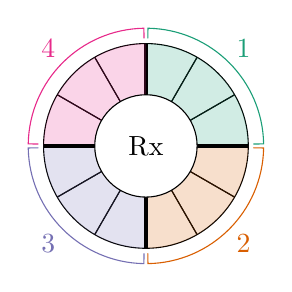
\begin{tikzpicture}[scale = 1.3]
\foreach \x in {0, 30, ..., 360}
	\draw ({cos(\x)}, {sin(\x)}) -- ({-cos(\x)}, {-sin(\x)});
\draw (0,0) circle [radius = 1cm];


\foreach[count = \i] \x/\c in {90/palette1, 0/palette2, -90/palette3, -180/palette4} {
	\draw[\c]
		({1.05 * cos (\x - 1)}, {1.05 * sin (\x - 1)})
		-- ({1.15 * cos (\x - 1)}, {1.15 * sin (\x - 1)})
		arc ({\x - 1}:{\x - 90 + 1}:1.15cm)
		-- ({1.05 * cos (\x - 90 + 1)}, {1.05 * sin (\x - 90 + 1)});

	\fill[opacity = 0.2, \c] (0,0) -- ({cos(\x)}, {sin(\x)})
		arc ({\x}:{\x - 90}:1cm) -- (0,0);

	\node[\c] at ({1.35 * cos (\x - 45)}, {1.35 * sin (\x - 45)}) {\i};

	\draw[very thick] (0,0) -- ({cos(\x)}, {sin(\x)});
}

\draw[black, fill = white] (0,0) circle [radius = 0.5cm]; % Poor man's \clip for intersecting regions
\node at (0,0) {Rx};

\end{tikzpicture}

\caption{División del anillo de recepción en cuatro segmentos fijos para los hilos.}
\label{fig:RingAssignment}
\end{wrapfigure}

Para evitar este problema, a cada hilo de lectura se le asigna un segmento fijo del anillo de recepción como en la \fref{fig:RingAssignment}. De esta forma cada hilo siempre accederá a los mismos descriptores, lo que permitirá incluir instrucciones de \textit{prefetch} para garantizar en la medida de lo posible que los datos a acceder estén siempre en la caché.

Esta asignación fija de segmentos del anillo también evita problemas de concurrencia, ya que no hay competición por acceso a los mismos recursos.

Por último, se minimiza el desorden en la lectura. Si todos los hilos leyesen los mismos descriptores, lo más probable es que los paquetes se copien en un orden distinto al que tenían cuando llegaron a la tarjeta. Sin embargo, de esta forma los hilos copian secuencialmente la mayor parte de los paquetes, y sólo se produciría desorden cuando haya dos o más hilos con paquetes pendientes al mismo tiempo. Con tasas bajas de paquetes por segundo, esto apenas ocurrirá durante pequeños intervalos de tiempo.

\subsection{Devolución ordenada de los descriptores leídos}

El siguiente problema a resolver es el de la devolución ordenada de los descriptores ya leídos y de las regiones de memoria correspondiente a la tarjeta, para que ésta los pueda reutilizar para los nuevos paquetes que lleguen. Es importante que esta devolución se realice por lotes al ser más eficiente. Además, ha de ser secuencial: no se pueden dejar atrás descriptores sin devolver ya que pueden provocar fallos de segmentación o la tarjeta los puede sobreescribir antes de tiempo.

Al segmentar el anillo de recepción, esta tarea se simplifica considerablemente y no son necesarios mecanismos de sincronización complejos. Cada hilo puede liberar los descriptores de su segmento por lotes sin problemas: la única restricción es que ya se hayan liberado todos los descriptores del segmento anterior.

La solución implementada es la siguiente. A cada hilo se le asignan dos variables, \texttt{can\_free} y \texttt{freed\_last\_rxd}. La primera variable indica si el hilo puede liberar sus descriptores, y la segunda si ya ha liberado el último de los descriptores de su segmento. A la hora de liberar los descriptores, se hace la primera comprobación sobre \texttt{can\_free}: si es 1, se liberan sin problemas. Además, si se llega al último descriptor, \texttt{freed\_last\_rxd} se pone a 1 y \texttt{can\_free} a 0 (hay que esperar, de nuevo, a que el segmento anterior libere sus descriptores).

Si, por otra parte, \texttt{can\_free} es 0, se lee la variable \texttt{freed\_last\_rxd} del segmento previo. Si es 1, indica que ya se pueden liberar los descriptores del segmento actual, así que se resetea su valor a 0 y \texttt{can\_free} se pone a 1. Es necesario que esta comprobación se haga sólo cuando \texttt{can\_free} sea 0. El pseudocódigo de este procedimiento se puede ver en el \fref{lst:AlgoritmoDescriptores}.

\begin{algorithm}[hbtp]
\begin{algorithmic}
\Function{free\_descriptors}{thread, descr}
\State prev $\gets$ previous\_thread\_of(thread)
	\If{can\_free[thread] == 0 \&\& freed\_last\_rxd[prev] == 1}
		\State freed\_last\_rxd[prev] $\gets$ 0
		\State can\_free[thread] $\gets$ 1
	\EndIf

	\If{can\_free[thread] == 1}
		\State release\_to\_NIC(descr)

		\If{is\_last\_in\_segment(descr, thread)}
			\State freed\_last\_rxd[prev] $\gets$ 1
			\State can\_free[thread] $\gets$ 0
		\EndIf
	\EndIf
\EndFunction
\end{algorithmic}
\caption{Algoritmo de liberación de descriptores}
\label{lst:AlgoritmoDescriptores}
\end{algorithm}

La única técnica de concurrencia usada es que la variable \texttt{freed\_last\_rxd} ha de ser atómica, de tal forma que su valor está constantemente sincronizado entre todos los hilos y no hay posibilidad de que un hilo la lea mientras otro está escribiendo su valor.

\subsection{Copia al \textit{buffer} intermedio de HPCAP}

\subsection{Hilos}
\label{sec:Hilos}

Varias posibilidades:

\begin{enumerate}
\item Separación del \textit{buffer} de la tarjeta en $n$ partes, cada hilo sólo se preocupa de una de esas partes. La tasa efectiva se reduce a $40 / n$ Gbps por hilo. El problema es que el anillo de la tarjeta se separa en paquetes y el buffer de HPCAP en bytes, así que un segmento de la tarjeta no tiene por qué corresponderse con otro segmento en el buffer.
\item Múltiples hilos escribiendo en el mismo buffer y leyendo del mismo anillo(s). Aquí habría que investigar una forma de sincronización eficiente, usando colas sin bloqueos. Un ejemplo interesante a leer es \href{http://disruptor.googlecode.com/files/Disruptor-1.0.pdf}{Disruptor}. Habría que investigar más bibliografía.
\item Como variación del anterior, múltiples hilos escribiendo en el mismo buffer pero leyendo de segmentos separados del anillo. Así quizás podemos evitar problemas de concurrencia a tasas bajas.
\end{enumerate}

Relacionado con las tasas bajas, una posibilidad con prioridad muy baja es mirar si se puede plantear creación dinámica de hilos según la tasa de recepción, de tal forma que entre el buffer y la creación dinámica se puedan ahorrar recursos en instalaciones con tasa suficientemente baja y sólo con picos de 40Gbps.

\section{Filtrado}

Estudiar filtros hardware y posibilidad de filtros software para reducir la tasa de tráfico recibida por la aplicación en espacio de usuario.

\section{Almacenamiento y selección de información}

Realizar un estudio teórico de necesidades de almacenamiento según tasa a la que queramos almacenar, viendo productos existentes en el mercado y calculando coste del sistema.

Estudiar si el driver puede realizar un prefiltrado de información en tiempo de recepción, extrayendo sólo ciertos campos de cada paquete. La extracción no debe de ser muy compleja y probablemente tenga que limitarse a extraer ciertos rangos fijos de bytes.

\section{Herramientas adicionales}

\textit{hpcap-test, hpcap-benchmark}.

\chapter{Pruebas}

\section{Caso base: ¿hasta dónde llega la arquitectura básica?}

\begin{figure}[btp]
\inputgnuplot{gnuplot/simple-arch-max-rate}
\caption[Capacidad de una arquitectura básica de captura]{Una medida de la capacidad base de la tarjeta: tasa máxima que se alcanza sin perder paquetes en función del tamaño de paquetes.}
\label{fig:SimpleArch:MaxRate}
\end{figure}

Dadas las limitaciones del \textit{hardware}, está claro que un único hilo de recepción no será suficiente para hacer la recepción a 40 Gbps. Aun así, es necesario realizar las pruebas en esta arquitectura simple para establecer una base sobre la que comparar y medir mejoras.

Tal y como se ve en la \fref{fig:SimpleArch:MaxRate}, sólo se llega a la tasa máxima de captura a partir de los 1250 bytes de tamaño de paquete. Para tamaños pequeños se observa el mismo comportamiento que con la versión original de HPCAP \citep{MorenoTFM2012}, donde para tamaños cercanos al mínimo (64 bytes) no se llegaba a la tasa máxima de 10 Gbps. En nuestro caso, para ese mismo tamaño se llega a una tasa de 7.6 Gbps.

Así mismo, sobre esta arquitectura básica se ha comprobado el efecto de las marcas de tiempo (\textit{timestamp}) obtenidas a través de la tarjeta o a través del reloj \textit{software} del \textit{kernel} Linux. El rendimiento en ambos casos es prácticamente el mismo.


\chapter{Conclusiones}

\appendix

\printnoidxglossaries
\cleardoublepage

\nocite{*}
\bibliography{hpcap40g}{}

\cleardoublepage
\printindex

\end{document}
